\documentclass[aspectratio=169]{beamer}

\usetheme[titleformat=regular,numbering=none,progressbar=frametitle]{metropolis}

% colour scheme
\definecolor{nclBlue}{HTML}{003A65}
\definecolor{nclRed}{HTML}{D91A35}
\definecolor{grey}{rgb}{0.52, 0.52, 0.51}
\definecolor{red}{rgb}{0.7, 0.11, 0.11}
\definecolor{blue}{rgb}{0.0, 0.0, 0.55}
\definecolor{green}{rgb}{0.0, 0.42, 0.24}

% beamer
\setbeamercovered{transparent}
\setbeamercovered{invisible}
\setbeamercolor{progress bar}{fg=nclRed}
\setbeamercolor{frametitle}{bg=nclBlue}
\setbeamercolor{background canvas}{bg=white}
\setbeamercolor{block body}{bg=gray!30}
\setbeamercolor{block title}{bg=nclBlue,fg=white}
\setbeamercolor{palette primary}{fg=white, bg=nclBlue}
\linespread{1.5}

% packages
\usepackage{graphicx}
\usepackage{booktabs}
\usepackage{amssymb}
\usepackage{pifont}
\usepackage{textcomp}
\usepackage{xcolor}
\usepackage{url}
\usepackage{xspace}
\usepackage{amsmath}
\usepackage{mathspec}
\usepackage[font=footnotesize]{caption}
\usepackage{subcaption}
% Thin fonts
\setsansfont[BoldFont={Fira Sans}, Numbers={OldStyle}]{Fira Sans Light}
\setmathsfont(Digits)[Numbers={Lining, Proportional}]{Fira Sans Light}

% Thick fonts
% \setsansfont[BoldFont={Fira Sans SemiBold}, Numbers={OldStyle}]{Fira Sans}
% \setmathsfont(Digits)[Numbers={Lining, Proportional}]{Fira Sans Book}

% commands
\newcommand{\tDelta}{\textsf{Delta}\xspace}

% tikz configuration
\usetikzlibrary{shapes.geometric, arrows}
\usetikzlibrary{arrows, positioning, shapes}
\usetikzlibrary{decorations.pathmorphing}
\usetikzlibrary{calc}
\tikzstyle{vertex} = [circle, minimum width=15pt,draw,inner sep=0pt]
\tikzstyle{mini_vertex} = [circle, minimum width=15pt,draw,inner sep=0pt]
\tikzstyle{server} = [rectangle, rounded corners,minimum width=3cm,minimum height=4cm,draw=black]
\tikzstyle{mini_server} = [rectangle, rounded corners,minimum width=1.5cm,minimum height=1.9cm,draw=black]
\tikzstyle{local} = [thick,->,>=stealth]
\tikzstyle{dist} = [thick,dashed,->,>=stealth]
\tikzstyle{bignode}=[draw, circle, minimum width=70pt,align=center]

\tikzstyle{big_vertex} = [circle, minimum width=50pt,draw,inner sep=0pt]

\def\record(#1,#2,#3,#4,#5,#6){
  \node (v) [draw,black,minimum height=0.9cm,minimum width=1cm,text width=0.2\linewidth,xshift=-7cm,align=center,yshift=#1cm] {#2};

  \node (b) [draw,black,minimum height=0.9cm,minimum width=15.9cm,text width=0.2\linewidth,xshift=2.85cm,yshift=#1cm] {};

  \draw[thick,->] (v) -- (b);

  \node (i1)  [draw,black,minimum height=0.6cm,minimum width=2cm,xshift=-3.1cm,text width=0.25\linewidth,yshift=#1cm,align=center] {#3};

  \node (i2)  [draw,black,minimum height=0.6cm,minimum width=2cm,xshift=1.9cm,right of=i1,yshift=0cm,text width=0.25\linewidth,align=center] {#4};

  \node (i3)  [draw,black,minimum height=0.6cm,minimum width=2cm,xshift=1.9cm,right of=i2,text width=0.25\linewidth,yshift=0cm,align=center] {#5};

  \node (i4)  [draw,black,minimum height=0.6cm,minimum width=2cm,xshift=1.9cm,right of=i3,text width=0.25\linewidth,yshift=0cm,align=center] {#6};

}

        \def\greenRecord(#1,#2,#3,#4,#5,#6){
  \node (v) [draw,black,minimum height=0.9cm,minimum width=1cm,text width=0.2\linewidth,xshift=-7cm,align=center,yshift=#1cm] {#2};

  \node (b) [draw,black,minimum height=0.9cm,minimum width=15.9cm,text width=0.2\linewidth,xshift=2.85cm,yshift=#1cm] {};

  \draw[thick,->] (v) -- (b);

  \node (i1)  [draw,black,minimum height=0.6cm,minimum width=2cm,xshift=-3.1cm,text width=0.25\linewidth,yshift=#1cm,align=center] {#3};

  \node (i2)  [draw,black,minimum height=0.6cm,minimum width=2cm,xshift=1.9cm,right of=i1,yshift=0cm,text width=0.25\linewidth,align=center,fill=green!30] {#4};

  \node (i3)  [draw,black,minimum height=0.6cm,minimum width=2cm,xshift=1.9cm,right of=i2,text width=0.25\linewidth,yshift=0cm,align=center] {#5};

  \node (i4)  [draw,black,minimum height=0.6cm,minimum width=2cm,xshift=1.9cm,right of=i3,text width=0.25\linewidth,yshift=0cm,align=center] {#6};

}

        \def\greenRecordB(#1,#2,#3,#4,#5,#6){
  \node (v) [draw,black,minimum height=0.9cm,minimum width=1cm,text width=0.2\linewidth,xshift=-7cm,align=center,yshift=#1cm] {#2};

  \node (b) [draw,black,minimum height=0.9cm,minimum width=15.9cm,text width=0.2\linewidth,xshift=2.85cm,yshift=#1cm] {};

  \draw[thick,->] (v) -- (b);

  \node (i1)  [draw,black,minimum height=0.6cm,minimum width=2cm,xshift=-3.1cm,text width=0.25\linewidth,yshift=#1cm,align=center] {#3};

  \node (i2)  [draw,black,minimum height=0.6cm,minimum width=2cm,xshift=1.9cm,right of=i1,yshift=0cm,text width=0.25\linewidth,align=center] {#4};

  \node (i3)  [draw,black,minimum height=0.6cm,minimum width=2cm,xshift=1.9cm,right of=i2,text width=0.25\linewidth,yshift=0cm,align=center,fill=green!30] {#5};

  \node (i4)  [draw,black,minimum height=0.6cm,minimum width=2cm,xshift=1.9cm,right of=i3,text width=0.25\linewidth,yshift=0cm,align=center] {#6};

}


\def\spaceRecord(#1){
  \node (v) [black,minimum height=0.9cm,minimum width=1cm,text width=0.2\linewidth,xshift=-7cm,align=center,yshift=#1cm] {$\vdots$};
  \node (b) [black,minimum height=0.9cm,minimum width=15.9cm,text width=0.2\linewidth,xshift=1.4cm,yshift=#1cm] {};
  \node (i1)  [black,minimum height=0.6cm,minimum width=2cm,xshift=-3.1cm,text width=0.3\linewidth,yshift=#1cm,align=center] {$\vdots$};
  \node (i2)  [black,minimum height=0.6cm,minimum width=2cm,xshift=1.9cm,right of=i1,yshift=0cm,text width=0.3\linewidth,align=center] {$\vdots$};
  \node (i3)  [minimum height=0.6cm,minimum width=2cm,xshift=1.9cm,right of=i2,yshift=0cm,align=center] {$\vdots$};
  \node (i4)  [minimum height=0.6cm,minimum width=2cm,xshift=1.9cm,right of=i3,yshift=0cm,align=center] {$\vdots$};
}


\title[]{Preserving Reciprocal Consistency in \\ Distributed Graph Databases}

\author[Waudby \& Ezhilchelvan \& Webber \& Mitrani]{\underline{\emph{Jack Waudby}}$^{1}$, Paul Ezhilchelvan$^{1}$, Jim Webber$^{2}$ \& Isi Mitrani$^{1}$}
\institute[NCL]
{
  $^{1}$Newcastle University\\
  $^{2}$Neo4j
}
\date{April 27, 2020}


\begin{document}

\begin{frame}
\maketitle
\begin{tikzpicture}[overlay, remember picture]
  \node[above left=2.8cm and 1.852cm of current page.south east]{
\includegraphics[width=3cm]{images/logo_newcastle_uni.png}};
  \node[above left=1.2cm and 1.852cm of current page.south east]{
\includegraphics[width=3cm]{images/logo_neo4j.png}};
\end{tikzpicture}
\end{frame}


\setcounter{framenumber}{0}
\metroset{numbering=counter}

\begin{frame}
  \frametitle{Property Graph}
  \begin{itemize}
  \item Graph databases model data as a \emph{property graph}
  \item Vertices represent entities and edges the relationships between entities
  \item Edges are \textbf{always} directional
  \end{itemize}
  \begin{figure}
    \centering
    \begin{tikzpicture}[node distance=2cm]
  \node (v1) [big_vertex,xshift=0cm,yshift=0cm] {\small{\texttt{a:\textcolor{green}{Person}}}};
  \node (v2) [big_vertex,xshift=5cm,yshift=0cm] {\small{\texttt{b:\textcolor{green}{Book}}}};
  \node [below of=v1,yshift=1cm] {\small{\texttt{\textcolor{red}{name}:Tolkien}}};
  \node [below of=v2,yshift=1cm] {\small{\texttt{\textcolor{red}{title}:The Hobbit}}};
  \draw [thick,->,>=stealth] (0.8,0)  -- node [midway,above] {:\textcolor{green}{\small{\texttt{WROTE}}}} (4.2,0);
\end{tikzpicture}

    \caption{Vertices connected by an edge}
  \end{figure}
\end{frame}

\begin{frame}
  \frametitle{Storage Layer Representation}
  \begin{itemize}
  \item In the storage layer,
    \begin{itemize}
    \item edge directionality does \textbf{not} exist
    \item connected vertices store information about each other
    \end{itemize}
  \item Bidirectional edge traversal speeds up query performance
  \end{itemize}
  \begin{figure}
    \centering
    \begin{tikzpicture}[node distance=2cm,scale=0.6,every node/.style={transform shape}]

  \greenRecord(
  0,
  \small{\texttt{a:Person}},
  \small{\texttt{name:Tolkien}},
  $\boldsymbol{\rightarrow}$ \textbf{\small{\texttt{wrote b}}},
  \texttt{edge},
  \texttt{edge}
  );

  \greenRecordB(
  -1,
  \small{\texttt{b:Book}},
  \texttt{property},
  \small{\texttt{title:The \hspace{-0.15cm} Hobbit}},
  $\boldsymbol{\leftarrow}$ \textbf{\small{\texttt{written by a}}},
  \texttt{edge}
  );

  \record(-2,
  \small{\texttt{vertex id}},
  \texttt{property},
  \texttt{property},
  \texttt{edge},
  \texttt{edge}
  );


  \spaceRecord(-2.7)

  \record(-3.6,
  \small{\texttt{vertex id}},
  \texttt{property},
  \texttt{edge},
  \texttt{edge},
  \texttt{edge}
  );

\end{tikzpicture}

    \caption{Edge storage layer representation}
  \end{figure}
\end{frame}

\begin{frame}
  \frametitle{Reciprocal Consistency}
  \centering
  When the adjacency list edge pointers for a given edge refer to each other in a complementary manner, that edge is \textbf{\emph{reciprocally consistent}}
\end{frame}

\begin{frame}
  \frametitle{Distributed Graph Databases}
  \centering
  Partition graph across machines in a cluster
  \begin{figure}[h!]
  \centering
  \resizebox{0.6\textwidth}{!}{
    \begin{tikzpicture}[node distance=2cm]
      \node (s1) [server,label=$S_i$] {};
      \node (s2) [server, right of=s1,xshift=2cm,yshift=2cm,label=$S_j$] {};
      \node (s3) [server, right of=s1,xshift=6cm,label=$S_k$] {};

      \node (v1) [vertex,xshift=-0.5cm,yshift=-1.5cm] {};
      \node (v2) [vertex, above of=v1,xshift=-0.3cm,yshift=1cm] {};
      \node (v3) [vertex, above of=v1,xshift=0.6cm] {};
      \node (v4) [vertex, below right of=v3,xshift=-0.5cm,yshift=-0.3cm] {};
      \node (v5) [vertex, above right of=v3,xshift=-0.6cm,yshift=-0.5cm] {};
      \node (v6) [vertex, right of=v5,xshift=0.3cm,yshift=0.8cm] {};
      \node (v7) [vertex, below of=v6, xshift=1cm,yshift=0.4cm] {};
      \node (v8) [vertex, right of=v4, yshift=-0.3cm,xshift=4.5cm] {};
      \node (v9) [vertex, above of=v8,xshift=-0.4cm,yshift=-0.5cm] {};
      \node (v10) [vertex, above of=v9,xshift=-2.5cm,yshift=-0.3cm] {};
      \node (v11) [vertex, right of=v9,yshift=0.5cm,xshift=-0.3cm] {};
      \node (v12) [vertex, above of=v11,yshift=-1cm,xshift=-1cm] {};
      \node (v13) [vertex, above right of=v6,yshift=-0.4cm,xshift=-0.1cm] {};
      \draw [local] (v2) -- (v1);
      \draw [local] (v1) -- (v3);
      \draw [local] (v3) -- (v2);
      \draw [local] (v2) -- (v5);
      \draw [local] (v1) -- (v4);
      \draw [local] (v5) -- (v4);
      \draw [dist] (v5) -- (v6);
      \draw [dist] (v4) -- (v7);
      \draw [dist] (v8) -- (v4);
      \draw [local] (v8) -- (v9);
      \draw [local] (v9) -- (v11);
      \draw [local] (v10) -- (v7);
      \draw [dist] (v10) -- (v12);
      \draw [dist] (v12) -- (v13);
      \draw [local] (v10) -- (v6);
      \draw [dist] (v10) -- (v11);
      \draw [local] (v13) -- (v10);
      \draw [local] (v11) -- (v12);
    \end{tikzpicture}
  }
  \caption{Partitioned graph}
\end{figure}

\end{frame}

\begin{frame}
  \frametitle{Distributed Graph Databases}
\begin{center}
  A degree of concurrency control is needed for ensuring reciprocal consistency of distributed edges
  \end{center}
\end{frame}

\begin{frame}
  \frametitle{Reciprocal Inconsistency}
  Distributed edge $ab$ indicates \texttt{Tolkien} wrote \texttt{The Hobbit}
  \begin{figure}
    \centering
    \begin{tikzpicture}[node distance=2.2cm]
  \node (rect)  [draw,rounded corners,minimum width=3.5cm,minimum height=4cm,label=above:{$S_i$}] {};
  \node (rect)  [draw,rounded corners,minimum width=3.5cm,minimum height=4cm,label=above:{$S_j$},xshift=6cm] {};
  \node (v1) [big_vertex,xshift=0cm,yshift=0cm] {\small{\texttt{a:\textcolor{green}{Person}}}};
  \node (v2) [big_vertex,xshift=6cm,yshift=0cm] {\small{\texttt{b:\textcolor{green}{Book}}}};
  \node [below of=v1,yshift=1cm] {\small{\texttt{\textcolor{red}{name}:Tolkien}}};
  \node [below of=v2,yshift=1cm] {\small{\texttt{\textcolor{red}{title}:The Hobbit}}};
  \draw [thick,dashed,->,>=stealth] (0.9,0)  -- node [midway,above] {:\textcolor{green}{\small{\texttt{WROTE}}}} (5.1,0);
\end{tikzpicture}
    \caption{Distributed edge}
  \end{figure}
\end{frame}

\begin{frame}
  \frametitle{Reciprocal Inconsistency}
  \begin{itemize}
  \item $T_x$ deletes the edge
  \item $T_y$ appends a property \textcolor{red}{\texttt{year}}
  \end{itemize}

  \begin{figure}
    \centering
    \begin{tikzpicture}
      \draw [thick,<-,>=stealth] (0,0) -- (0,4) node[anchor=south] {$S_i$};
      \draw [thick,<-,>=stealth] (4,0) -- (4,4) node[anchor=south] {$S_j$};
      \draw [thick,<-,>=stealth] (0,1) -- (4,3)  node[right] {$T_y$};
      \draw [thick,->,>=stealth] (0,3.6) node[left] {$T_x$} -- (4,1.2);
    \end{tikzpicture}
  \end{figure}
\end{frame}

\begin{frame}
  \frametitle{Reciprocal Inconsistency}
  The distributed edge is now reciprocally inconsistent
  \begin{figure}
    \centering
    \begin{tikzpicture}[node distance=2cm]
  \node (v1) [big_vertex,xshift=0cm,yshift=0cm] {\small{\texttt{a:\textcolor{green}{Person}}}};

  \node (v2) [big_vertex,xshift=5cm,yshift=0cm] {\small{\texttt{b:\textcolor{green}{Book}}}};

  \node [below of=v1,yshift=1cm] {\small{\texttt{\textcolor{red}{name}:Tolkien}}};
  \node [below of=v2,yshift=1cm] {\small{\texttt{\textcolor{red}{title}:The Hobbit}}};

  \draw [thick,->,>=stealth] (0.8,0)  -- node [midway,above] {:\textcolor{green}{\small{\texttt{WROTE}}}} node [midway,below] {\small{\texttt{\textcolor{red}{year} = 1937}}} (2.4,0);
\end{tikzpicture}

    \caption{Reciprocally inconsistent distributed edge}
  \end{figure}
\end{frame}

\begin{frame}
  \frametitle{Reciprocal Inconsistency}
Storage representation consists of two inconsistent unidirectional edges

\begin{figure}
\centering
\begin{subfigure}{.5\textwidth}
  \centering
  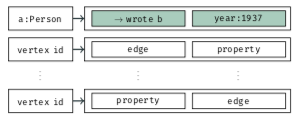
\includegraphics[width=.9\linewidth]{./images/si}
  \caption{$S_i$}
  \label{fig:sub1}
\end{subfigure}%
\begin{subfigure}{.5\textwidth}
  \centering
  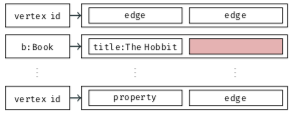
\includegraphics[width=.9\linewidth]{./images/sj}
  \caption{$S_j$}
  \label{fig:sub2}
\end{subfigure}
\caption{Storage representation}
\label{fig:test}
\end{figure}
\end{frame}

\begin{frame}
  \frametitle{Reciprocal Inconsistency}
  \begin{itemize}
  \item Reciprocally inconsistent edges are the source for \emph{semantic corruption}
  \item Semantic corruption spreads until the database becomes \emph{operationally corrupt}
  \item \textbf{Motivated the design of a lightweight protocol that preserves reciprocal consistency}
  \end{itemize}
\end{frame}

\begin{frame}
  \frametitle{Protocol Design Considerations}
  Design Considerations:
  \begin{enumerate}
  \item Graph workloads exhibit high contention.
  \item Graph transactions tend to be long-lived than those in other databases.
  \end{enumerate}
\textbf{Protocol must permit multiple updates on the same record provided they are they are \textit{sufficiently} apart in time in ensure reciprocal consistency}
\end{frame}

\begin{frame}
  \frametitle{\tDelta Protocol}
  \begin{itemize}
  \item Fact: a transaction updating a distributed edge must update one edge pointer then \textbf{immediately} update the other.
  \item Rule: an update is permitted if the immediately preceding update was done at least $\Delta$ time before. Else, abort.
  \item Assumption: the time interval that elapses between completing at update at one end and starting at the other can be estimated, $\delta$. Choosing $\Delta > \delta$.
  \end{itemize}
\end{frame}

\begin{frame}
  \frametitle{\tDelta Protocol: Example}
  \begin{center}
    \textbf{\small{Rule: an update is permitted if the preceding update was done at least $\Delta$ time before. Else, abort}}
  \end{center}
  \begin{figure}[h!]
    \centering
    \begin{tikzpicture}
      \uncover<2->{
        \draw [black,<-,>=stealth] (-3,1) -- (-3,3) node [label=above:{time}] {};
        \draw [black,<-,>=stealth] (0,0) -- (0,4) node [label=above:{$S_i$}] {};
        \draw [black,<-,>=stealth] (4,0) -- (4,4)  node [label=above:{$S_j$}] {};
              \draw [white,<-,>=stealth] (7,1) -- (7,3) ;
      }
      \uncover<2->{
        \node [] at (-0.5,4) {$T_x$};
      }
      \uncover<3-6>{
        \draw [->,>=stealth] (0,3.5) -- (2,1.9);
      }
      \uncover<4->{
        \node [] at (4.5,3.3) {$T_y$};
      }
      \uncover<5-5>{
        \draw [->,>=stealth] (4,3.3) -- (2,2.9);
      }
      \uncover<6-8>{
        \draw [->,>=stealth] (4,3.5) -- (0,2.5);
      }
      \uncover<6-8>{
        \draw [<->,>=stealth] (-0.3,2.5) -- (-0.3,3.3);
        \node[] at (-0.8,3) {$< \Delta$};
        \node[] at (-1.5,2.5) {$T_y$ ABORTS};
      }
      \uncover<7->{
        \draw [->,>=stealth] (0,3.5)  -- (4,0.3);
      }
      \uncover<8-8>{
        \node[] at (6,1) {$T_x$ SUCCEEDS};
        \draw [<->,>=stealth] (4.3,0.3) -- (4.3,3.3);
        \node[] at (4.8,1.8) {$> \Delta$};
      }
    \end{tikzpicture}
  \end{figure}
\end{frame}

\begin{frame}
  \frametitle{\tDelta Protocol}
  \begin{itemize}
  \item Reciprocal consistency is preserved if the time taken to complete am update at one end and start at other end remains less than  $\Delta$
  \item If $\Delta$ is exceeded then reciprocal inconsistency can occur
  \item Setting a large $\Delta$ tends to preserve consistency but leads to more aborted transactions
  \end{itemize}
\end{frame}

\begin{frame}
  \frametitle{Performance Evaluation}
  Two metrics the following two metrics for various values of $\Delta$:
  \begin{itemize}
  \item Time taken for 10\% of a large database to be corrupt
    \item Number of transactions aborted per second
  \end{itemize}
\end{frame}

\begin{frame}
  \frametitle{Time until 10\% database corruption2 $\boldsymbol{log(U)}$ vs Transaction Arrival Rate $(\boldsymbol{\lambda})$}
  \begin{center}
    For $\Delta = 50ms$, time taken for 10\% database corruption is between to $1$-$75$ years
  \end{center}
    \begin{figure}[h!]
    \centering
    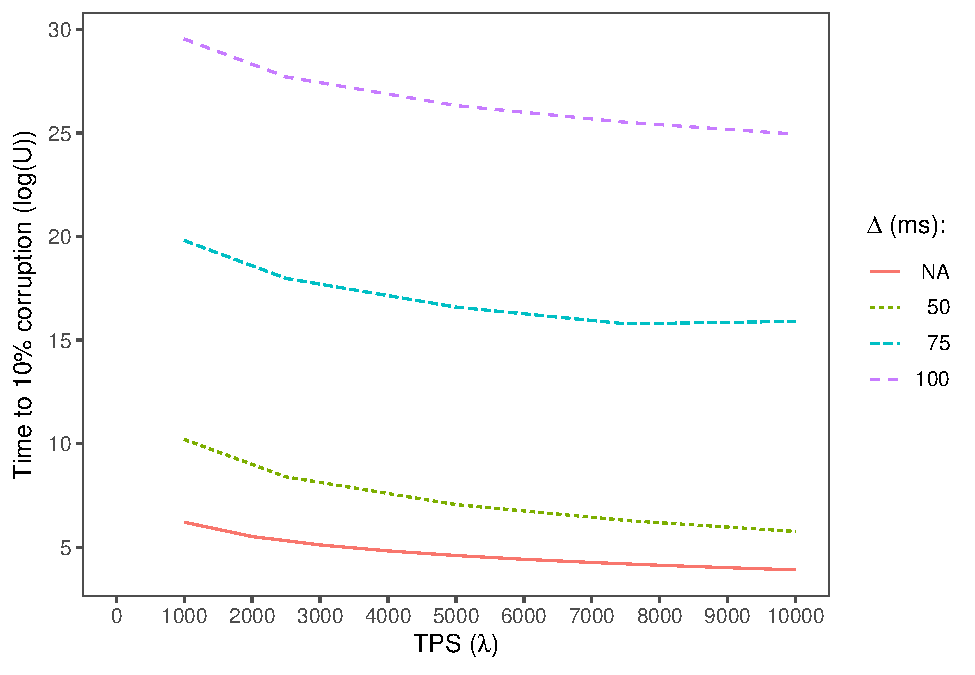
\includegraphics[scale=0.5]{./figures/delta}
  \end{figure}
\end{frame}

\begin{frame}
  \frametitle{Fraction of Aborts vs Transaction Arrival Rate $(\boldsymbol{\lambda})$}
  \begin{center}
    For $\Delta = 50 ms$, the fraction of aborts is between 1 − 5\%
  \end{center}
    \begin{figure}[h!]
    \centering
    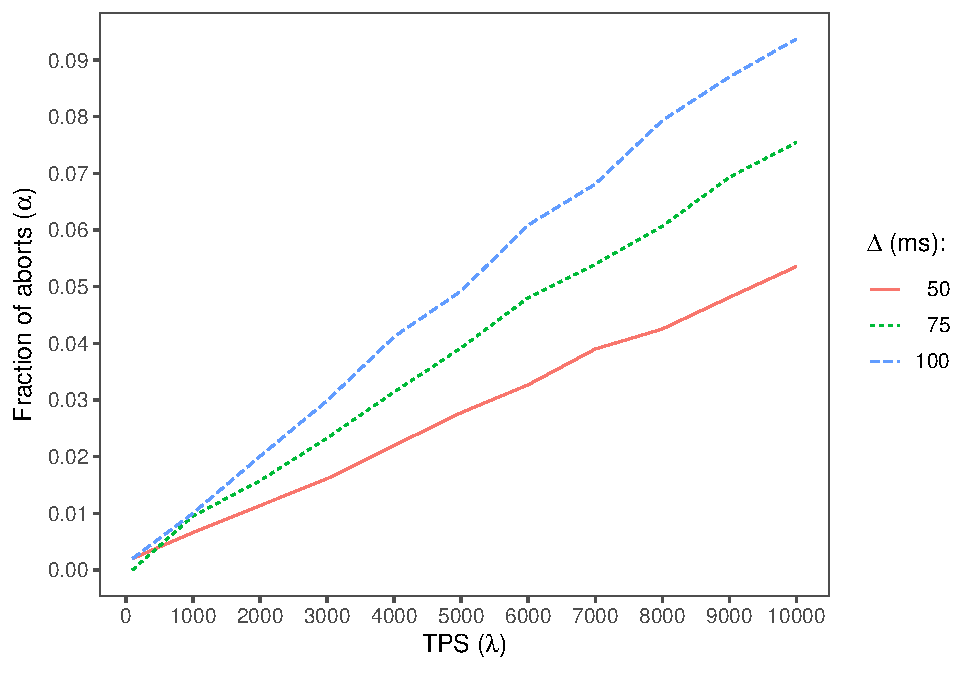
\includegraphics[scale=0.5]{./figures/aborts}
  \end{figure}
\end{frame}

\begin{frame}
  \frametitle{Summary}
  \begin{itemize}
  \item Lack of concurrency control can lead to reciprocally inconsistent edges
  \item Semantic corruption spreads quickly in a graph database
  \item \tDelta protocol prevents reciprocal inconsistency given the bound $\Delta$ in not violated
  \item \tDelta protocol significantly reduces the time until operational corruption at the cost of some aborts
  \end{itemize}
\end{frame}


% %------------------------------------------------
% % Problem 1: Reciprocal Consistency}
% % ------------------------------------------------



% \begin{frame}
%   \frametitle{Reciprocal Consistency Violation}
%   Two concurrent transactions:
%   \begin{itemize}
%   \item Mr Red requests to book the seat, $T_R$
%   \item Mr Blue requests to book the seat, $T_B$
%   \end{itemize}
% \end{frame}

% \begin{frame}
%   \frametitle{Reciprocal Consistency Violation}
%   \begin{figure}[h!]
%     \centering
%     \begin{tikzpicture}[node distance=2cm]
%       \uncover<1-> {
%         \draw [black,<-,>=stealth] (0,0) -- (0,4) node [] {};
%         \draw [black,<-,>=stealth] (4,0) -- (4,4) node [] {};
%         \draw [black,dashed,->,>=stealth] (0,4.1) node [label=above:{$S_1$}] {} -- node [midway,above] {$E$} (4,4.1) node [label=above:{$S_2$}] {};
%       }
%       \uncover<2-3> {
%         \draw [red,->,>=stealth] (0,3.6) node [label=left:{$T_R$}] {} -- (2,2.3);
%       }
%       \uncover<3-4> {
%         \draw [blue,->,>=stealth] (4,3) node [label=right:{$T_B$}] {} -- (2,2.1);
%       }
%       \uncover<4-> {
%         \draw [red,->,>=stealth] (0,3.6) node [label=left:{$T_R$}] {} -- (4,1);
%       }
%       \uncover<5-> {
%         \draw [blue,->,>=stealth] (4,3) node [label=right:{$T_B$}] {} -- (0,1.2);
%       }
%     \end{tikzpicture}
%     \caption{Concurrent transactions interleave and violate reciprocal consistency}
%   \end{figure}
% \end{frame}

% \begin{frame}
%   \frametitle{Reciprocal Consistency Violation}
%   \begin{figure}[h!]
%     \centering
%     \begin{tikzpicture}[node distance=7cm]
%       \node (n1) [bignode] {\texttt{Flight}};
%       \node (rect)  [draw,dashed,minimum width=3cm,minimum height=3cm,label=above:{$S_1$}] {};
%       \node (rect)  [draw,dashed,minimum width=3cm,minimum height=3cm,label,xshift=7cm,label=above:{$S_2$}] {};
%       \node (n2) [bignode, right of=n1] {\texttt{Seat}};
%       \draw [local] (n1) to[out=0,in=-180]  node[below] {\texttt{:BOOKED}} (n2);

%       \uncover<2-> {
%       \node (q1) [rectangle, minimum width=0.6cm,minimum height=0.6cm,draw=black,xshift=0cm,yshift=-2.5cm] {\textit{Mr Blue Booked In Seat}};
%       \node (q2) [rectangle,minimum width=0.6cm,minimum height=0.6cm,draw=black,xshift=7cm,yshift=-2.5cm] {\textit{Mr Red Booked In Seat}};
%       \draw [<->,dashed](q1) -- (q2);
%       \draw [<->,dashed](q1) -- (q2);
%       \coordinate (a) at (4,-2);
%       \coordinate (b) at (3,-3);
%       \coordinate (c) at (3,-2);
%       \coordinate (d) at (4,-3);
%       \draw [very thick,red] ($ (a) $) -- ($ (b) $);
%       \draw [very thick,red] ($ (c) $) -- ($ (d) $);
%     }
%     \end{tikzpicture}
%     \caption{Reciprocal inconsistent distributed edge}
%   \end{figure}
% \end{frame}

% % \begin{frame}
% %   \frametitle{Reciprocal Consistency Violation}
% %   \begin{figure}[h!]
% %     \centering
% %     \begin{tikzpicture}[node distance=2cm]
% %       \uncover<1->{
% %         \draw [black,<-,>=stealth] (4.5,0) -- (4.5,4) node [] {};
% %         \draw [red,->,>=stealth] (4.5,2.2) node [label=left:{$T_x$}] {} -- (6.5,1);
% %         \draw [blue,->,>=stealth] (6.5,2.7) node [label=right:{$T_y$}] {} -- (4.5,1.2);
% %         \draw [black,<-,>=stealth] (6.5,0) -- (6.5,4) node [] {};
% %         \draw [black,dashed,->,>=stealth] (4.5,4.1) node [label=above:{$S_1$}] {} -- node [midway,above] {$E$} (6.5,4.1) node [label=above:{$S_2$}] {};
% %       }
% %       \uncover<2->{
% %         \draw [black,<-,>=stealth] (9,0) -- (9,4) node [] {};
% %         \draw [red,->,>=stealth] (9,3.5) node [label=left:{$T_x$}] {} -- (11,1);
% %         \draw [blue,->,>=stealth] (9,2.8) node [label=left:{$T_y$}] {} -- (11,2);
% %         \draw [black,<-,>=stealth] (11,0) -- (11,4) node [] {};
% %         \draw [black,dashed,->,>=stealth] (9,4.1) node [label=above:{$S_1$}] {} -- node [midway,above] {$E$} (11,4.1) node [label=above:{$S_2$}] {};
% %       }
% %     \end{tikzpicture}
% %     \caption{Possible interleaving of concurrent transactions that violate reciprocal consistency}
% %   \end{figure}
% % \end{frame}

% \begin{frame}
%   \frametitle{Distributed Edge Reciprocal Consistency}
%   \begin{itemize}
%     \uncover<1->{
%   \item Without concurrency control, distributed edges can become reciprocally inconsistent
%     \begin{itemize}
%     \item A distributed edge's reciprocal information is separated by the network
%     \end{itemize}
%   }
%   \uncover<2->{
%   \item Reciprocal inconsistency is a source of corruption\footnotemark
%   }
%   \uncover<3->{
%   \item No known concurrency control protocol exists specific to graph databases and maintaining reciprocal consistency
%     }
%     \end{itemize}
%     \footnotetext[3]{Ezhilchelvan, P. et al, \textit{On the degradation of distributed graph databases with eventual consistency}. European Performance Engineering Workshop 2018.}
% \end{frame}


% \begin{frame}
%   \frametitle{Our Solution: Collision Detection}
%   \begin{itemize}
%     \uncover<1->{
%     \item Carefully abort transaction(s)
%     }
%     \uncover<2->{
%     \item No centralized control or synchronized clock
%     }
%     \uncover<3->{
%     \item Permits interleavings that preserve reciprocal consistency
%     }
%   \end{itemize}
% \end{frame}

% \begin{frame}
%   \frametitle{Collision Detection General Rules}
%   \begin{itemize}
%     \uncover<1->{
%     \item Updates are initially provisional
%     }
%     \uncover<2->{
%     \item Transactions distinguish between their first and second updates using labels
%     }
%     \uncover<3->{
%     \item When a transaction attempts to update a given record, it can identify all other transactions that have earlier updated that record provisionally
%     }
%   \end{itemize}
% \end{frame}

% \begin{frame}
%   \frametitle{Interference-free Update}
%   \begin{figure}[h!]
%     \centering
%     \begin{tikzpicture}
%       \uncover<1->{
%         \draw [black,<-,>=stealth] (-3,1) -- (-3,3) node [label=above:{time}] {};
%         \draw [white,<-,>=stealth] (7,1) -- (7,3) ; %placeholder to balance picture
%         \draw [black,<-,>=stealth] (0,0) -- (0,4) ;
%         \draw [black,<-,>=stealth] (4,0) -- (4,4) ;
%         \draw [black,dashed,->,>=stealth] (0,4.5) node [label=above:{$e_{out}$ in $S_1$}] {} -- (4,4.5) node [label=above:{$e_{in}$ in $S_2$}] {};
%       }
%       \uncover<2->{
%         \node [] at (-0.5,4) {\textcolor{red}{$T_R$}};
%       }
%       \uncover<3->{
%         \node [] at (-0.5,3.5) {\textcolor{red}{$1$}};
%       }
%       \uncover<3->{
%         \draw [red,->,>=stealth] (0,3.5) node [] {} -- (4,0.3) node (TX) [] {};
%       }
%       \uncover<4->{
%         \node [] at (4.5,0.3) {\textcolor{red}{$2$}};
%       }
%     \end{tikzpicture}
%   \end{figure}

% \end{frame}

% \begin{frame}
%   \frametitle{Collision Detection}
%   \begin{center}
%     \textbf{Rule: For any ``1'' seen, there must be a ``2'' in the opposite end. Else, abort}
%   \end{center}
%   \begin{figure}[h!]
%     \centering
%     \begin{tikzpicture}
%       \uncover<2->{
%         \draw [black,<-,>=stealth] (-3,1) -- (-3,3) node [label=above:{time}] {};
%         \draw [black,<-,>=stealth] (0,0) -- (0,4) ;
%         \draw [black,<-,>=stealth] (4,0) -- (4,4) ;
%         \draw [black,dashed,->,>=stealth] (0,4.5) node [label=above:{$e_{out}$ in $S_1$}] {} -- (4,4.5) node [label=above:{$e_{in}$ in $S_2$}] {};
%         \draw [white,<-,>=stealth] (7,1) -- (7,3) ; %placeholder to balance picture
%       }
%       \uncover<2->{
%         \node [] at (-0.5,4) {\textcolor{red}{$T_R$}};
%       }
%       \uncover<3->{
%         \node [] at (-0.5,3.5) {\textcolor{red}{$1$}};
%       }
%       \uncover<4-11>{
%         \draw [red,->,>=stealth] (0,3.5) -- (2,1.9);
%       }
%       \uncover<5-10>{
%         \node [] at (-0.5,2.6) {\textcolor{blue}{$T_B$}};
%       }
%       \uncover<6-10>{
%         \node [] at (-0.5,2.1) {\textcolor{blue}{$1$}};
%       }
%       \uncover<7-7>{
%         \draw [blue,->,>=stealth] (0,2.1) -- (2,1.8);
%       }
%       \uncover<8-10>{
%         \draw [blue,->,>=stealth] (0,2.1) -- (4,1.5);
%         \node [] at (4.5,1.5) {\textcolor{blue}{$2$}};
%       }
%       \uncover<9-9>{
%         \node [] at (6,2) {$T_R$'s 2 is missing};
%       }
%       \uncover<10-10>{
%         \node[] at (6,2) {$T_B$ ABORTS};
%       }
%       \uncover<12->{
%         \draw [red,->,>=stealth] (0,3.5)  -- (4,0.3);
%       }
%       \uncover<13->{
%         \node [] at (4.5,0.3) {\textcolor{red}{$2$}};
%       }
%       \uncover<14->{
%         \node[] at (6,2) {$T_R$ SUCCEEDS};
%         }
%     \end{tikzpicture}
%   \end{figure}
% \end{frame}

% %------------------------------------------------
% %Problem 2: Edge-Order Consistency
% % ------------------------------------------------

% \begin{frame}
%   \frametitle{Edge-Order Consistency}
%   A second consistency problem related to distributed edges:
%   \begin{itemize}
%     \uncover<2->{
%     \item Consider 2 transactions that update $2$ or more of the \textit{same} distributed edges
%     }
%     \uncover<3->{
%     \item Each update is reciprocally consistent
%     }
%     \uncover<4->{
%     \item Then if $T_R$ updates before $T_B$ on a given edge then this order should be preserved across all edges
%     }
%   \end{itemize}
% \end{frame}

% \begin{frame}
%   \frametitle{Edge-Order Consistency Violation}
%   Consider two edges,
%   \begin{figure}[h!]
%     \centering
%     \resizebox{1\textwidth}{!}{
%       \begin{tikzpicture}[node distance=5.2cm]
%         \node[] at (2.6,2.5) {\large{$E$}};
%         \node[] at (13,2.5) {\large{$E'$}};
%         \node (n1) [bignode] {\texttt{Flight}};
%         \node (rect)  [draw,dashed,minimum width=3cm,minimum height=3cm,label=above:{$S_1$}] {};
%         \node (rect)  [draw,dashed,minimum width=3cm,minimum height=3cm,label,xshift=5.2cm,label=above:{$S_2$}] {};
%         \node (n2) [bignode, right of=n1] {\texttt{Seat}};
%         \draw [local] (n1) to[out=0,in=-180]  node[below] {\small{\texttt{:AVAILABLE}}} (n2);
%         \node (q1) [rectangle, minimum width=0.6cm,minimum height=0.6cm,draw=black,xshift=0cm,yshift=-2cm] {\textit{Seat Available In Flight}};
%         \node (q2) [rectangle,minimum width=0.6cm,minimum height=0.6cm,draw=black,xshift=5.2cm,yshift=-2cm] {\textit{In Flight Seat Available}};
%          \draw [<->,dashed](q1) -- (q2);

%         \node (n3) [bignode, right of=n2] {\texttt{Hotel}};
%         \node (n4) [bignode, right of=n3] {\texttt{Room}};
%         \draw [local] (n3) to[out=0,in=-180]  node[below] {\small{\texttt{:AVAILABLE}}} (n4);
%         \node (q3) [rectangle, minimum width=0.6cm,minimum height=0.6cm,draw=black,xshift=10.4cm,yshift=-2cm] {\textit{Room Available In Hotel}};
%         \node (q4) [rectangle,minimum width=0.6cm,minimum height=0.6cm,draw=black,xshift=15.6cm,yshift=-2cm] {\textit{In Hotel Room Available}};
%         \node (rect)  [draw,dashed,minimum width=3cm,minimum height=3cm,xshift=15.6cm,label=above:{$S_4$}] {};
%         \node (rect)  [draw,dashed,minimum width=3cm,minimum height=3cm,label,xshift=10.4cm,label=above:{$S_3$}] {};
%         \draw [<->,dashed](q3) -- (q4);

%       \end{tikzpicture}
%     }
%     \caption{Two distributed edges}
%   \end{figure}
% \end{frame}

% \begin{frame}
%   \frametitle{Edge-Order Consistency Violation}
%   Two concurrent transactions by a travel agent:
%   \begin{itemize}
%   \item Requests to book room and seat for Mr Red, $T_R$
%   \item Requests to book room and seat for Mr Blue, $T_B$
%   \end{itemize}
% \end{frame}

% \begin{frame}
%   \frametitle{Edge-Order Consistency Violation}
%   \begin{figure}[h!]
%     \centering
%     \begin{tikzpicture}
%       \uncover<1->{

%         \draw [black,->,>=stealth] (0,0) -- (10,0) node [label=below:{$time$}] {};
%         \draw [black,-,>=stealth] (2,4) node [label={[red]left:{$T_R$}}] {} -- (8,4);
%         \draw [black,-,>=stealth] (8,4.1) node [] {} -- (8,3.9);
%         \draw [black,-,>=stealth] (2,4.1) node [] {} -- (2,3.9);
%         \draw [black,-,>=stealth] (4,2) node [label={[blue]left:{$T_B$}}] {} -- (7,2);
%         \draw [black,-,>=stealth] (4,2.1) node [] {} -- (4,1.9);
%         \draw [black,-,>=stealth] (7,2.1) node [] {} -- (7,1.9);
%       }
%       \uncover<2->{
%         \draw [black,dashed] (2.5,0) node [label=below:{$t_1$}] {} -- (2.5,4) node [label=above:{$E$}] {};
%       }
%       \uncover<3->{
%         \draw [black,dashed] (4.5,0) node [label=below:{$t_2$}] {} -- (4.5,2) node [label=above:{$E$}] {};
%       }
%       \uncover<4->{

%         \draw [black,dashed] (6.5,0) node [label=below:{$t_3$}] {} -- (6.5,2) node [label=above:{$E'$}] {};
%       }
%       \uncover<5->{

%         \draw [black,dashed] (7.5,0) node [label=below:{$t_4$}] {} -- (7.5,4) node [label=above:{$E'$}] {};
%       }
%       \uncover<6->{
%         \draw (8.3,2) node [label=right:{$E : T_R \rightarrow T_B$}] {} ;
%         \draw (8.3,1.5) node [label=right:{$E' : T_B \rightarrow T_R$}] {} ;
%         \draw (8.3,1) rectangle (11,2.5);
%       }
%     \end{tikzpicture}
%     \caption{Edge-order consistency violation}
%   \end{figure}
% \end{frame}

% \begin{frame}
%   \frametitle{Edge-Order Consistency Violation}
%   \begin{figure}[h!]
%     \centering
%     \resizebox{1\textwidth}{!}{
%       \begin{tikzpicture}[node distance=5cm]
%         % edge labels
%         \node[] at (2.5,3) {\large{$E$}};
%         \node[] at (12.5,3) {\large{$E'$}};
%         % edge 1: flight -> seat
%         \node (n1) [bignode] {\texttt{Flight}};
%         \node (n2) [bignode, right of=n1] {\texttt{Seat}};
%         % edge 1: servers
%         \node (rect)  [draw,dashed,minimum width=3cm,minimum height=3cm,label=above:{$S_1$}] {};
%         \node (rect)  [draw,dashed,minimum width=3cm,minimum height=3cm,label,xshift=5cm,label=above:{$S_2$}] {};
%         % edge 1
%         \draw [local] (n1) to[out=0,in=-180]  node[below] {\texttt{:BOOKED}} (n2);
%         % edge 1 information
%         \node (q1) [rectangle, minimum width=0.6cm,minimum height=0.6cm,draw=black,xshift=0cm,yshift=-2cm] {\textcolor{red}{\textit{Mr Red Booked Seat}}};
%         \node (q2) [rectangle,minimum width=0.6cm,minimum height=0.6cm,draw=black,xshift=5cm,yshift=-2cm] {\textcolor{red}{\textit{Mr Red Booked Seat}}};
%         \draw [<->,dashed](q1) -- (q2);

%         % edge 2: hotel -> room
%         \node (n3) [bignode, right of=n2] {\texttt{Hotel}};
%         \node (n4) [bignode, right of=n3] {\texttt{Room}};
%         \draw [local] (n3) to[out=0,in=-180]  node[below] {\texttt{:BOOKED}} (n4);
%         \node (q3) [rectangle, minimum width=0.6cm,minimum height=0.6cm,draw=black,xshift=10cm,yshift=-2cm] {\textcolor{blue}{\textit{Mr Blue Booked Room}}};
%         \node (q4) [rectangle,minimum width=0.6cm,minimum height=0.6cm,draw=black,xshift=15cm,yshift=-2cm] {\textcolor{blue}{\textit{Mr Blue Booked Room}}};
%         \node (rect)  [draw,dashed,minimum width=3cm,minimum height=3cm,xshift=15cm,label=above:{$S_4$}] {};
%         \node (rect)  [draw,dashed,minimum width=3cm,minimum height=3cm,label,xshift=10cm,label=above:{$S_3$}] {};
%         \draw [<->,dashed](q3) -- (q4);

%       \end{tikzpicture}
%     }
%     \caption{Edge-order consistency violation}
%   \end{figure}
% \end{frame}

% \begin{frame}
%   \frametitle{Our Solution: Order Arbitration}
%   \begin{itemize}
%   \uncover<1->{
%   \item Transactions collect predecessors from each update
%   }
%   \uncover<2->{
%   \item Centralized arbiter maintains some global state
%   }
%   \uncover<3->{
%   \item Global state used to detect edge-order violations
%   }
%   \uncover<4->{
%   \item Offending transactions are aborted
%   }
%   \end{itemize}
% \end{frame}

% \begin{frame}
%   \frametitle{Order Arbitration}
%     \begin{center}
%       \textbf{Rule: Collect predecessors after every successful update}
%     \end{center}
%   \begin{figure}[h!]
%     \centering
%     \begin{tikzpicture}
%       \uncover<1->{
%         \draw [black,<-,>=stealth] (0,0) -- (0,4) ;
%         \draw [black,<-,>=stealth] (3,0) -- (3,4) ;
%         \draw [black,dashed,->,>=stealth] (0,4.5) node [label=above:{$S_1$}] {} -- node [midway,above] {$E$} (3,4.5) node [label=above:{$S_2$}] {};
%         \draw [black,<-,>=stealth] (7,0) -- (7,4) ;
%         \draw [black,<-,>=stealth] (10,0) -- (10,4) ;
%         \draw [black,dashed,->,>=stealth] (7,4.5) node [label=above:{$S_3$}] {} -- node [midway,above] {$E'$} (10,4.5) node [label=above:{$S_4$}] {};
%       }
%       \uncover<2->{
%         \draw [blue,->,>=stealth] (0,3.2) node (TXS) [label=left:{\small{$T_B$}}] {} -- (3,3);
%         \draw [red,->,>=stealth] (3,3.6) node (TXS) [label=right:{\small{$T_R$}}] {} -- (0,3.4);
%         \draw (3.1, 2.8) node [label=right:{\small{\textcolor{black}{$T_B : \{{T_R}\}$}}}] {};
%         \draw (3.2,2.3) rectangle (5,3.2);
%       }
%       \uncover<3->{
%         \draw [blue,->,>=stealth] (7,2.3) node [label=left:{\small{$T_B$}}] {} -- (10,1.8);
%         \draw [red,->,>=stealth] (7,1.8) node [label=left:{\small{$T_R$}}] {} -- (10,1.2) ;
%         \draw (10.1, 0.8) node (TXS) [yshift=-1cm,label=right:{\small{\textcolor{black}{$T_R : \{{T_B}\}$}}}] {};
%         \draw (10.2,-0.6) rectangle (12,0.3);
%       }
%       \uncover<4->{
%         \draw [->,decorate,decoration={snake,amplitude=.4mm,segment length=2mm,post length=1mm}]
%         (10.2,1.8) node[above,xshift=1cm, yshift=0.3cm] {ARBITER} -- (11,1.8);
%         \draw [->,decorate,decoration={snake,amplitude=.4mm,segment length=2mm,post length=1mm}]
%         (10.2,1.2)   -- (11,1.2);
%       }
%     \end{tikzpicture}
%   \end{figure}
% \end{frame}

% \begin{frame}
%   \frametitle{Order Arbitration}
%       \begin{center}
%       \textbf{Rule: If transaction exists in hit list, abort. Else, merge predecessors into hit list}
%     \end{center}
%   \begin{figure}[h!]
%     \centering
%     \begin{tikzpicture}
%       \uncover<1->{ % 1 arbiter
%         \node (s1) [server,label=$Arbiter$] {};
%       }
%       \uncover<2->{ % 2 hit list
%         \node (a) [rectangle, label=above:{$Hit \ List$}, minimum width=2cm,minimum height=1cm,draw=black,xshift=0cm,yshift=0cm] {$T_z$ ,$T_a$ {\uncover<7->{,$T_R$}}};
%       } % uncover T_R when T_B processed
%       \uncover<3->{ % 3 queue
%               \node (q) [rectangle, label=above:{$Queue$},left of=s1, minimum width=1cm,minimum height=1cm,draw=black,xshift=-4.5cm,yshift=0cm] {{\uncover<6->{$...$}}};
%               \node [rectangle, left of=s1, minimum width=1cm,minimum height=1cm,draw=black,xshift=-3.5cm,yshift=0cm] {{\uncover<5-8>{$T_R$}}};
%         \node [rectangle, left of=s1, minimum width=1cm,minimum height=1cm,draw=black,xshift=-2.5cm,yshift=0cm] {{\uncover<4-5>{$T_B$}}};
%         \node (q1) [rectangle, left of=s1, minimum width=1cm,minimum height=1cm,draw=black,xshift=-4.5cm,yshift=-1cm] {{\uncover<6->{$...$}}};
%         \node [rectangle, left of=s1, minimum width=1cm,minimum height=1cm,draw=black,xshift=-3.5cm,yshift=-1cm] {{\uncover<5-8>{$T_B$}}};
%         \node [rectangle, left of=s1, minimum width=1cm,minimum height=1cm,draw=black,xshift=-2.5cm,yshift=-1cm] {{\uncover<4-5>{$T_R$}}};
%         \node [left of=q,xshift=0.2cm,label=left:{\small{\textcolor{black}{$tnx.id$}}}] {};
%         \node [left of=q1,xshift=0.2cm,label=left:{\small{\textcolor{black}{$pred$}}}] {};
%       }
%       \uncover<4-4> {
%         \node[right=0.5cm of s1] {$T_B$ \textbf{ENTERS QUEUE}};
%       }
%       \uncover<5-5> {
%         \node[right=0.5cm of s1] {$T_R$ \textbf{ENTERS QUEUE}};
%       }
%       \uncover<6-8> {
%         \node[right=0.5cm of s1,yshift=1cm] {$T_B$ \textbf{PROCESSED}};
%       }
%       \uncover<7-8> {
%         \node[right=0.5cm of s1,yshift=0cm] {$T_R$ \textbf{ADDED TO HIT LIST}};
%       }
%       \uncover<8-8> {
%         \node[right=0.5cm of s1,,yshift=-1cm] {$T_B$ \textbf{SUCCEEDS}};
%       }
%       \uncover<9-> {
%         \node[right=0.5cm of s1,yshift=1cm] {$T_R$ \textbf{PROCESSED}};
%       }
%       \uncover<10-> {
%         \node[right=0.5cm of s1,yshift=0cm] {$T_R$ \textbf{IN HIT LIST}};
%       }
%       \uncover<11-> {
%         \node[right=0.5cm of s1,yshift=-1cm] {$T_R$ \textbf{ABORTS}};
%       }
%     \end{tikzpicture}
%   \end{figure}
% \end{frame}

% \begin{frame}
%   \frametitle{Order Arbitration Protocol}
%   If a transaction updates $1$ or more distributed edges:
%   \begin{itemize}
%     \uncover<1->{
%     \item Collect all predecessors
%     }
%     \uncover<2->{
%     \item Go to arbiter
%     }
%     \uncover<3->{
%     \item If not in hit list then proceed and enter predecessors into the hit list
%     }
%     \uncover<4->{
%     \item Else in hit list then abort
%     }
%   \end{itemize}
% \end{frame}

% \begin{frame}
%   \frametitle{Edge Concurrency Control Protocol Summary}
%     \begin{enumerate}
%     \item Collision detection: enforces \textbf{reciprocal consistency} for distributed edges
%     \item Order arbitration: enforces \textbf{edge-order consistency} between transactions
%     \end{enumerate}
% \end{frame}


% %------------------------------------------------
% % Performance Evaluation
% % ------------------------------------------------

% \begin{frame}
%   \frametitle{Performance Evaluation}
%   Performance measures of interest:
%   \begin{itemize}
%   \item Average number of transactions that are aborted
%   \item Load at the arbiter
%   \end{itemize}
% \end{frame}

% \begin{frame}
%   \frametitle{Evaluation Approach}
%   \begin{enumerate}
%   \item Developed approximate model
%   \item Measure accuracy of model through simulation
%   \end{enumerate}
% \end{frame}

% \begin{frame}
%   \frametitle{Parameters}
%   \begin{itemize}
%   \item Database size
%   \item Transaction arrival rate
%   \item Average updates per transaction
%   \item Average arbiter service time
%   \item Average network delay
%   \end{itemize}
% \end{frame}



% %------------------------------------------------
% % Numerical and Simulation Results
% % ------------------------------------------------

% \begin{frame}
%   \frametitle{Aborts per second $(\boldsymbol{R})$ vs Database Size $(\boldsymbol{N})$}
%   \begin{figure}[h!]
%     \centering
%     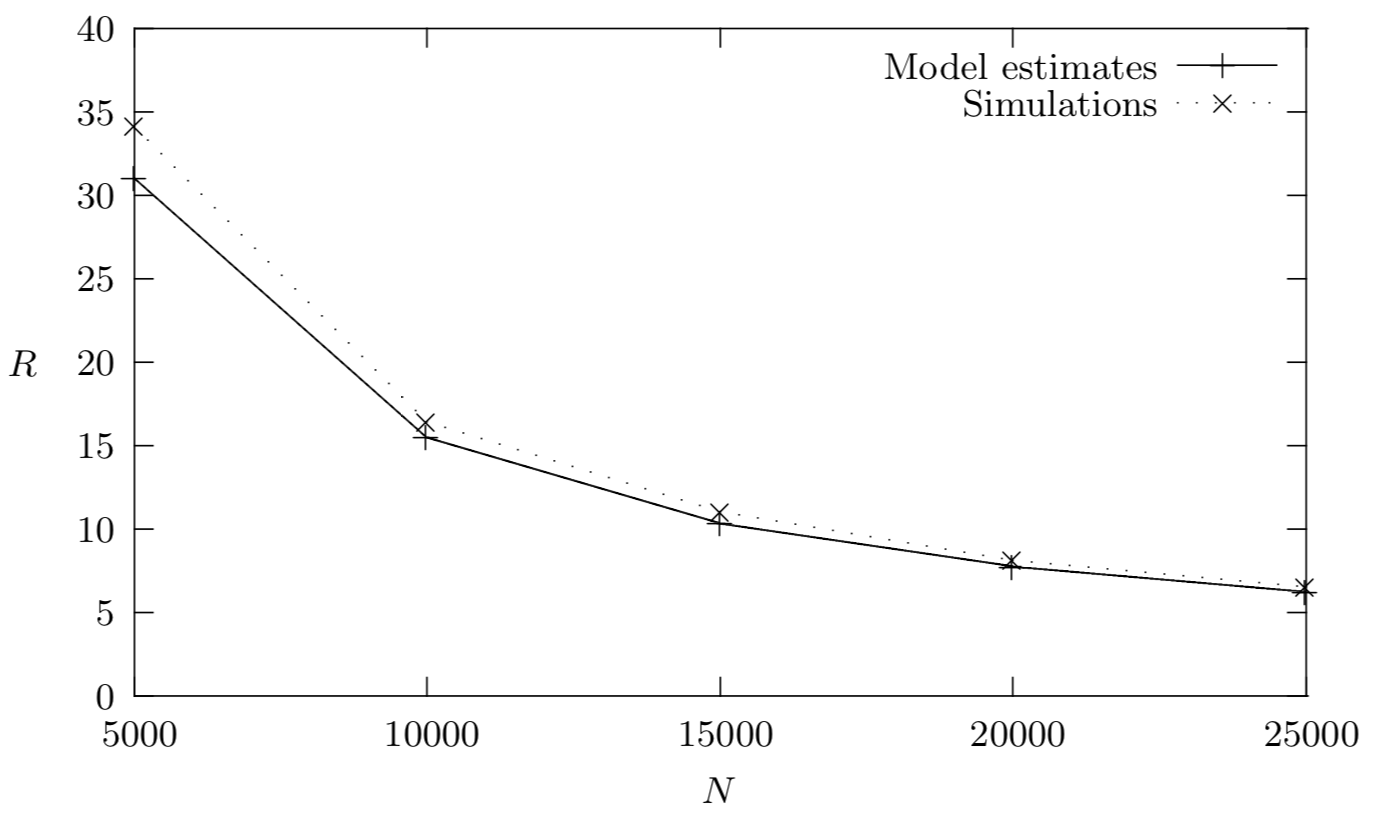
\includegraphics[scale=0.35]{images/varying_num_edges.png}
%     \caption{TPS $= 1000$, av updates/tnx $= 5$, av arbiter service time $= 10ms$, av network delay $=5ms$}
%   \end{figure}
% \end{frame}

% \begin{frame}
%   \frametitle{Aborts per second $(\boldsymbol{R})$ vs Transaction Arrival Rate $(\boldsymbol{\lambda})$}
%   \begin{center}
%     Arbiter queue unstable at $\sim1500$ TPS
%   \end{center}
%   \begin{figure}[h!]
%     \centering
%     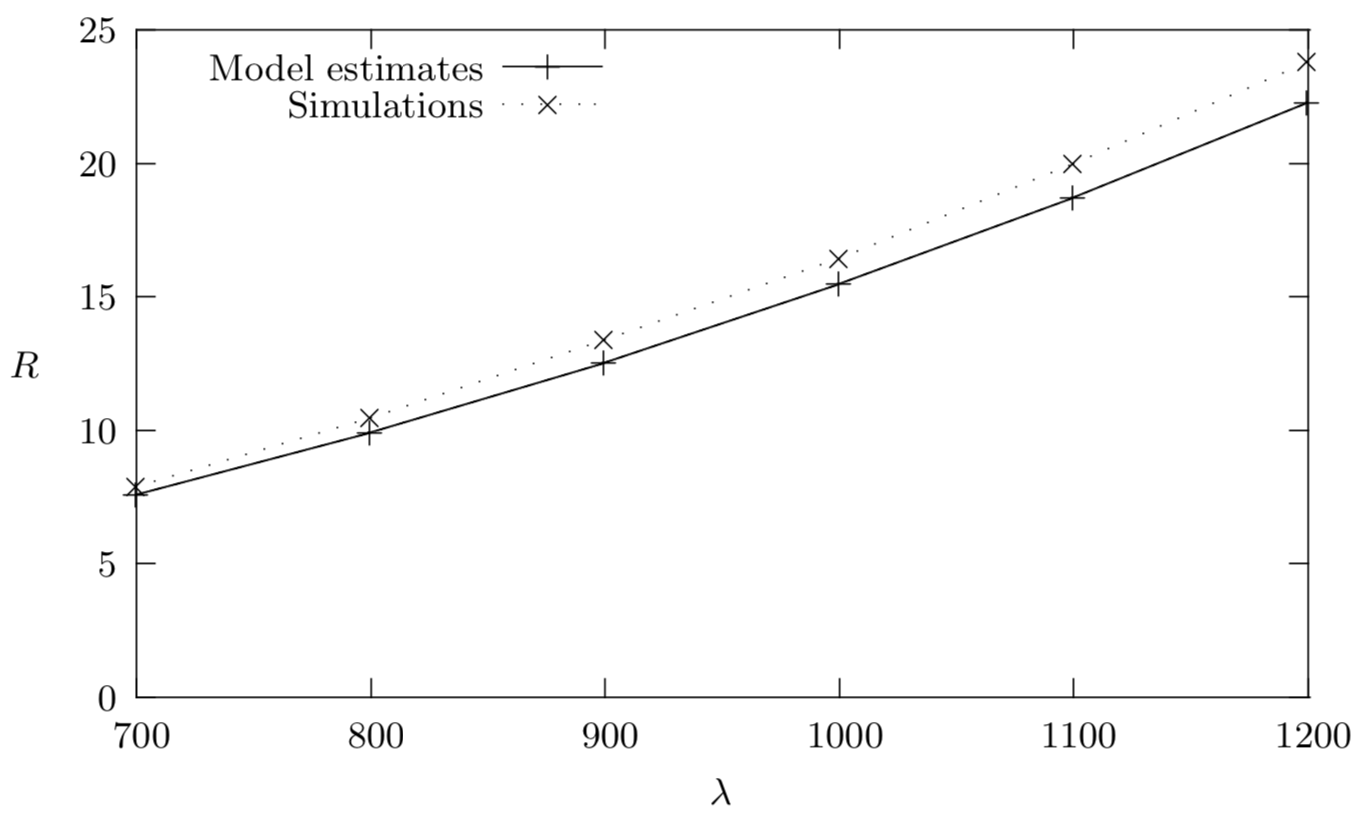
\includegraphics[scale=0.35]{images/varying_tnx_arrival_rate}
%     \caption{\textcolor{red}{size $= 10K$}, av updates/tnx $= 5$, av arbiter service time $= 10ms$, av network delay $=5ms$}
%   \end{figure}
% \end{frame}

% \begin{frame}
%   \frametitle{Aborts per second $(\boldsymbol{R})$ vs Transaction Arrival Rate $(\boldsymbol{\lambda})$}
%   \begin{center}
%     Arbiter queue unstable at $\sim 1100$ TPS
%   \end{center}
%   \begin{figure}[h!]
%     \centering
%     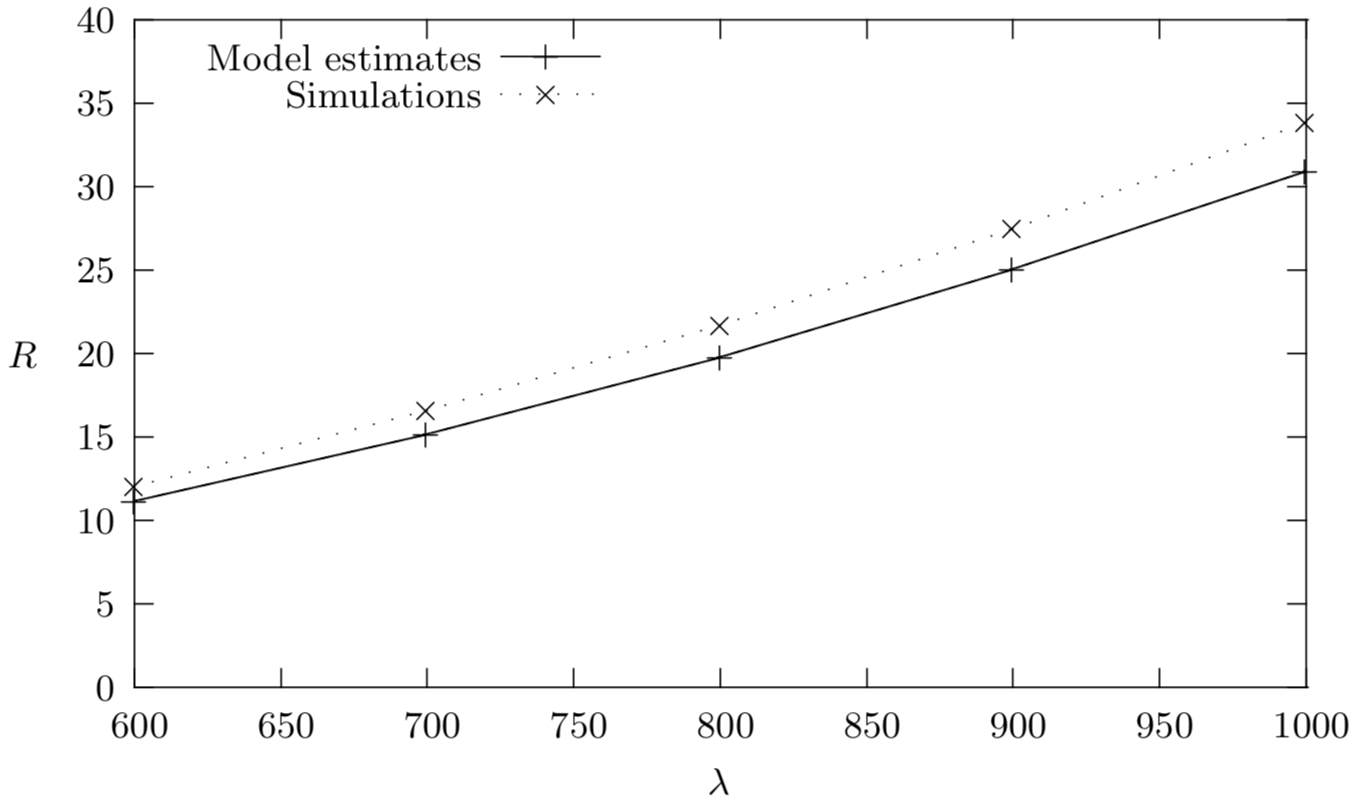
\includegraphics[scale=0.35]{images/larger_network_delay.png}
%     \caption{size $= 10K$, av updates/tnx $= 5$, av arbiter service time $= 10ms$, \textcolor{red}{av network delay $=10ms$}}
%   \end{figure}
% \end{frame}

% \begin{frame}
%   \frametitle{Aborts per second $(\boldsymbol{R})$ vs Transaction Arrival Rate $(\boldsymbol{\lambda})$}
%   \begin{center}
%     Arbiter queue unstable at $\sim 550$ TPS
%   \end{center}
%     \begin{figure}[h!]
%     \centering
%     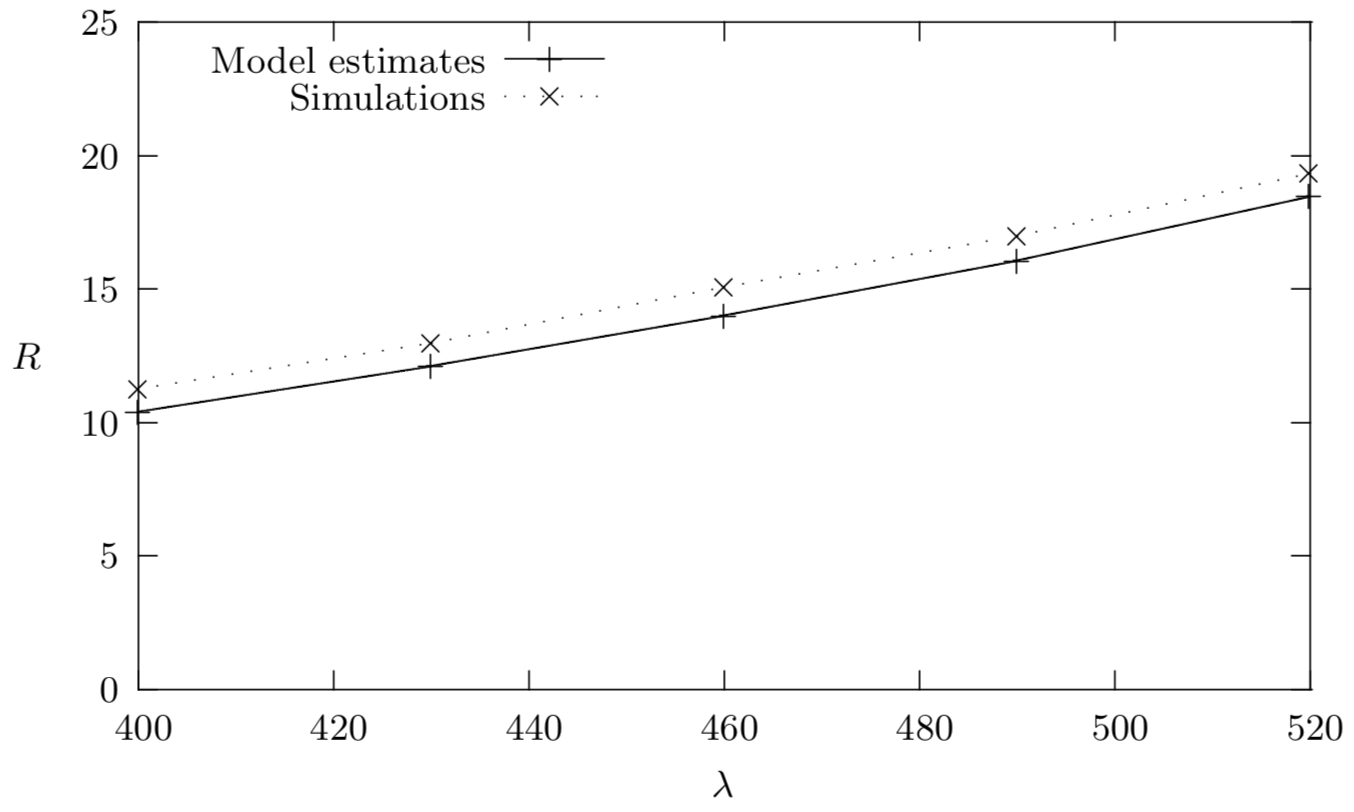
\includegraphics[scale=0.35]{images/varying_updates_per_tnx.png}
%         \caption{size $= 10K$, \textcolor{red}{av updates/tnx $= 10$}, av arbiter service time $= 10ms$, av network delay $=5ms$}
%   \end{figure}
% \end{frame}

% \begin{frame}
%   \frametitle{Summary and Future Work}
%   \begin{itemize}
%     \uncover<1->{
%     \item Model accuracy similar to simulations under a variety of parameter settings
%     }
%     \uncover<2->{
%     \item Between 1-4\% transactions are aborted
%     }
%     \uncover<3->{
%     \item Improve accuracy of simulation
%     }
%   \end{itemize}
% \end{frame}

% \begin{frame}[standout]
%  Thanks for listening! \\
%   \vspace{4mm}
%   Any Questions? \\
%   \vspace{4mm}
%   {\normalsize Email: \href{mailto:j.waudby2@newcastle.ac.uk}{j.waudby2@newcastle.ac.uk}} \\
%   {\normalsize Twitter: \href{https://twitter.com/waudberry_7}{@waudberry\_7}}
% \end{frame}

\end{document}
